\documentclass[preprintnumbers,amsmath,amssymb,superscriptaddress,twocolumn,showpacs]{revtex4-2}
\usepackage{graphicx}% Include figure files
\usepackage{dcolumn}% Align table columns on decimal point
\usepackage{bm}% bold math
\usepackage{physics}
\usepackage[caption=false]{subfig}



\def\sgn{\mathop{\rm sgn}}
\newcommand{\be}{\begin{equation}}
\newcommand{\ee}{\end{equation}}
\newcommand{\bea}{\begin{eqnarray}}
\newcommand{\eea}{\end{eqnarray}}

\begin{document}

\title{Relaxation of Dipolar-Coupled Spins in Transverse Fields : \\ The role of Double-flip Processes}

\author{C. Pellet-Mary$^1$, M. Perdriat$^1$, P. Huillery$^2$,  G. H\'etet} 

\affiliation{Laboratoire De Physique de l'\'Ecole Normale Sup\'erieure, \'Ecole Normale Sup\'erieure, PSL Research University, CNRS, Sorbonne Universit\'e, Universit\'e Paris Cit\'e , 24 rue Lhomond, 75231 Paris Cedex 05, France \\$^2$Univ Rennes, INSA Rennes, CNRS, Institut FOTON - UMR 6082, F-35000 Rennes, France}

\begin{abstract}
We study relaxation processes in dipolar-coupled negatively charged nitrogen vacancy (NV$^-$) centers under transverse electric fields and magnetic fields. Specifically, we uncover regimes where flip-flop, double-flip processes as well as mixing induced by local electric fields play a significant role in NV-NV cross-relaxation.
Our results are relevant for understanding decoherence in many-body spin systems as well as for high sensitivity magneto- and electro-metry with long-lived interacting solid-state spins. As a proof of principle, we present an orientation and microwave-free magnetometer based on cross-relaxation.
\end{abstract}

\maketitle

The electronic spin properties of the negatively charged nitrogen-vacancy (NV$^-$) center in diamond have given rise to a wealth of applications in nanoscale sensing and quantum information science thanks in part to the possibility to optically polarize and read-out its spin state under ambient conditions \cite{DOHERTY20131}. In particular, ensembles of NV centers are widely studied for their enhanced magnetic field sensing capabilities \cite{Acosta, TALLAIRE2020421,edmonds2021characterisation, chatzidrosos2021fiberized, Barry, Bauch} and as pristine platforms for observing many-body effects \citep{kucsko2018critical, ChoiNat, ZuYao, dwyer2021probing}. When the NV spin concentration reaches ppm values, spin depolarisation, or cross-relaxation (CR) takes place through a very rich many-body dynamics associated with disorder \citep{choi_observation_2017}. These mechanisms limit the efficiency of typical microwave based NV magnetometers, but quantum control techniques can be combined to surpass this interaction limit \citep{zhou2020quantum}. Further, CR mechanisms can be turned as a tool for magnetic field sensing \cite{akhmedzhanov_microwave-free_2017, akhmedzhanov_magnetometry_2019}. 
Spectral features in the photoluminescence (PL) indeed appear when the magnetic field crosses specific crystal planes where dipolar interactions are enhanced, leading to CR. The projected sensitivity of such magnetometers lie in the tens of pT$/\sqrt{\rm Hz}$  \cite{akhmedzhanov_microwave-free_2017}, on a par with the most sensitive microwave based NV magnetometers \cite{Wolf, Sturner}. 

Cross-relaxation features close to zero magnetic field have also been observed and could be deployed for higher sensitivity microwave-free magnetometry \cite{filimonenko2018weak, filimonenko2022manifestation}.
The CR contrast was indeed shown to be much larger in this zero-field limit \citep{jarmola_longitudinal_2015,  mrozek_longitudinal_2015} but all the relaxation mechanisms have not been identified.
Here, we study dipolar relaxation processes in ensembles of NV centers in the presence of small transverse electric and magnetic fields. Specifically, by employing magnetic field scans along specific crystalline directions, we find regimes where flip-flop, double-flip processes as well as mixing induced by local electric fields play a role. We also present an orientation and microwave-free magnetometer that employs double-flip processes in the dipolar interaction between NV centers.

\begin{figure}
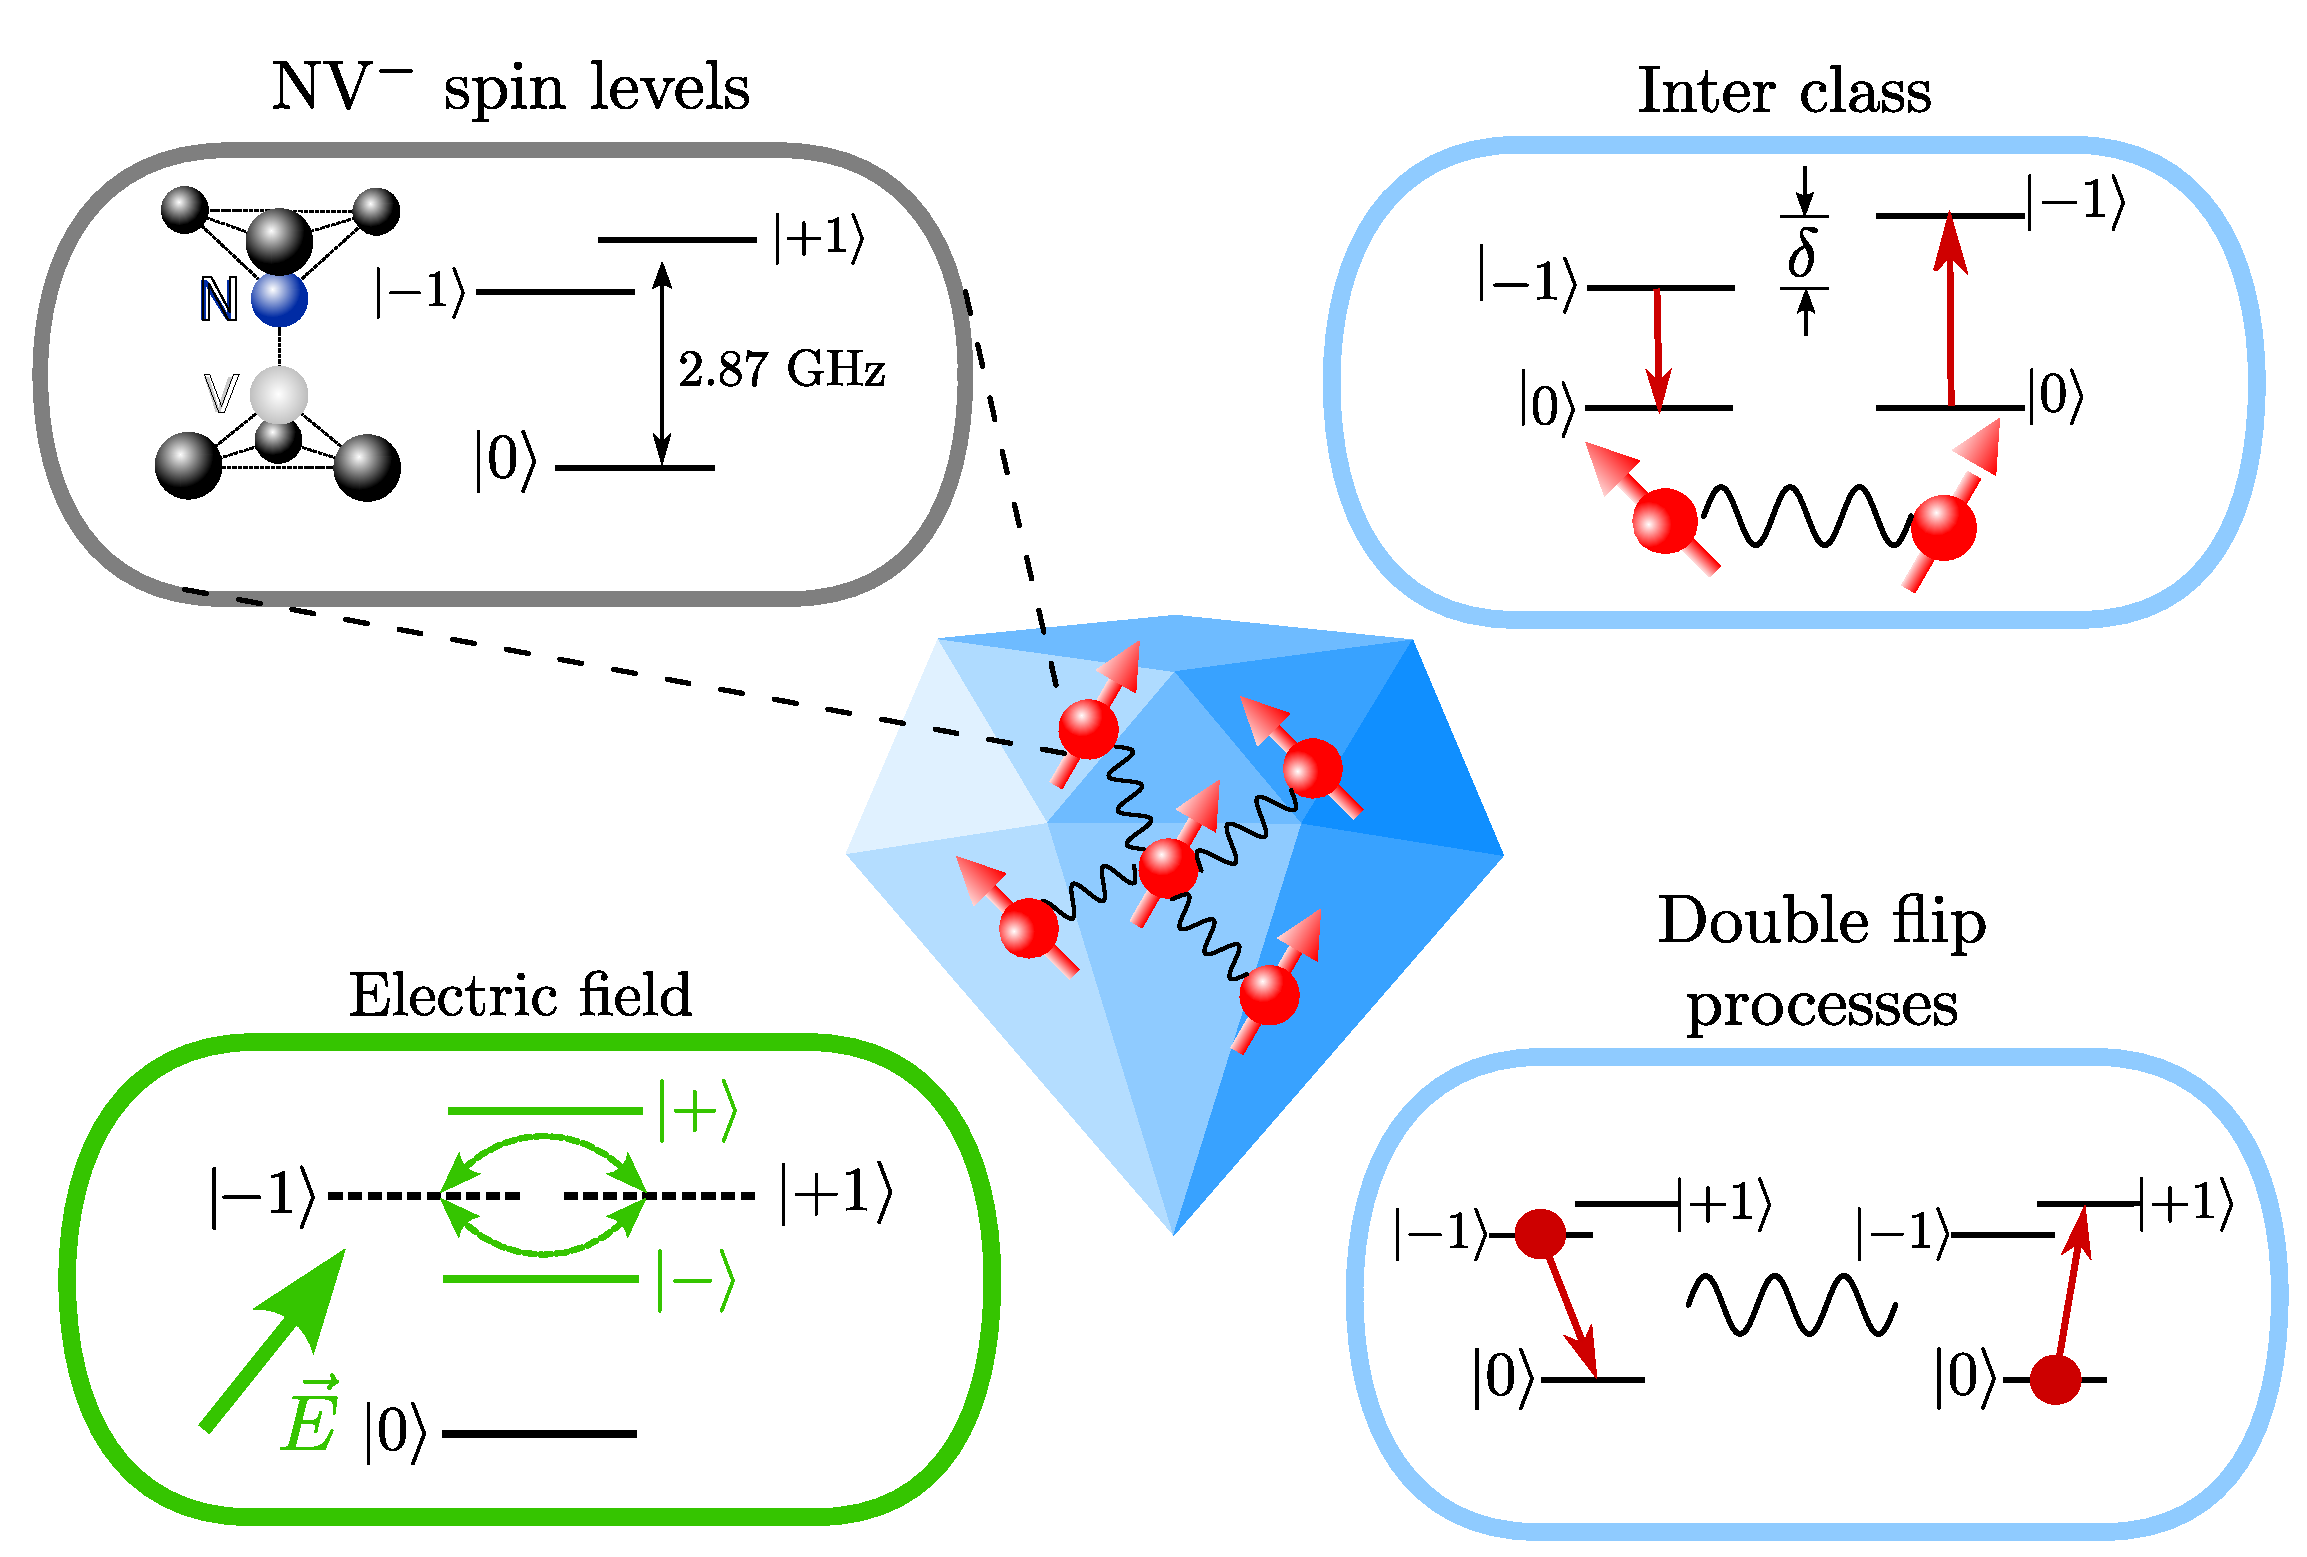
\includegraphics[width=0.45\textwidth]{shema_summary.pdf}
\caption{Schematics showing a diamond with interacting spins (central picture) as well as three processes that account for dipolar relaxation: flip-flop processes involving two different classes of NV centers, local electric field mixing and double-flip processes where two units of spin angular momentum are exchanged. }
\label{schema_intro}
\end{figure}

The electronic spin of NV center is a spin-1 system in the electronic ground state (see Fig. 1, top left panel), which can be optically polarized in the $\ket{m_s=0}$ state. The PL of this state is also larger than in the $\ket{m_s=\pm 1}$ states enabling spin-read out at room temperature \cite{DOHERTY20131}. The $\ket{m_s=\pm 1}$ spin states are separated from the $\ket{m_s=0}$ state by  $D = (2\pi) 2.87$ GHz so that when a resonant microwave or static transverse magnetic field is applied, the PL is reduced \citep{epstein2005anisotropic,lai2009influence}.  The processes that lead to depolarisation in strongly coupled spin-1 systems are depicted in Fig.~1. Flip-flop processes involving coupling between spins with identical or different orientations, or ``classes", are depicted in the top-right panel. They have already been shown to play a dominant role in dense ensembles of NV centers when $B \gtrsim 30$~G : tuning the difference $\delta$ between the different NV centers' spin states indeed result in a strong $T_1$ reduction \cite{choi_observation_2017}.  We will show here that double-flip up and down as well as mixing induced by local electric fields (cf. two bottom panels) can also give a significant contribution to the spin depolarization.

The experimental apparatus and the samples used in this study together with their nomenclature are presented in the supplementary material (SM) sec. II and III \citep{SI_low_filed_CR}\nocite{anishchik2015low, filimonenko2020weak, van1990electric, giri_coupled_2018, giri_selective_2019, Hall,jarmola_temperature-_2012}. 
%The nomenclature that we use indicates first the fabrication process: high pressure high temperature (HPHT) or chemical vapor deposition (CVD). 
%In the case of HPHT grown samples, these indications are followed by the size of the diamond particle in $\mu$m. 
Fig.  \ref{T1}-a) and b) show the change in PL as a function of a magnetic field applied {\it via} a homebuilt electromagnet for two diamond samples with a low and high concentration of NV$^-$ centers respectively (CVD-1 and HPHT-150-1). In both samples, we see a decrease in PL as the magnetic field amplitude increases. There is however a stark difference in the low magnetic field region where only high-density samples shows a drop in PL \citep{jarmola_longitudinal_2015,  mrozek_longitudinal_2015}. 
\begin{figure}
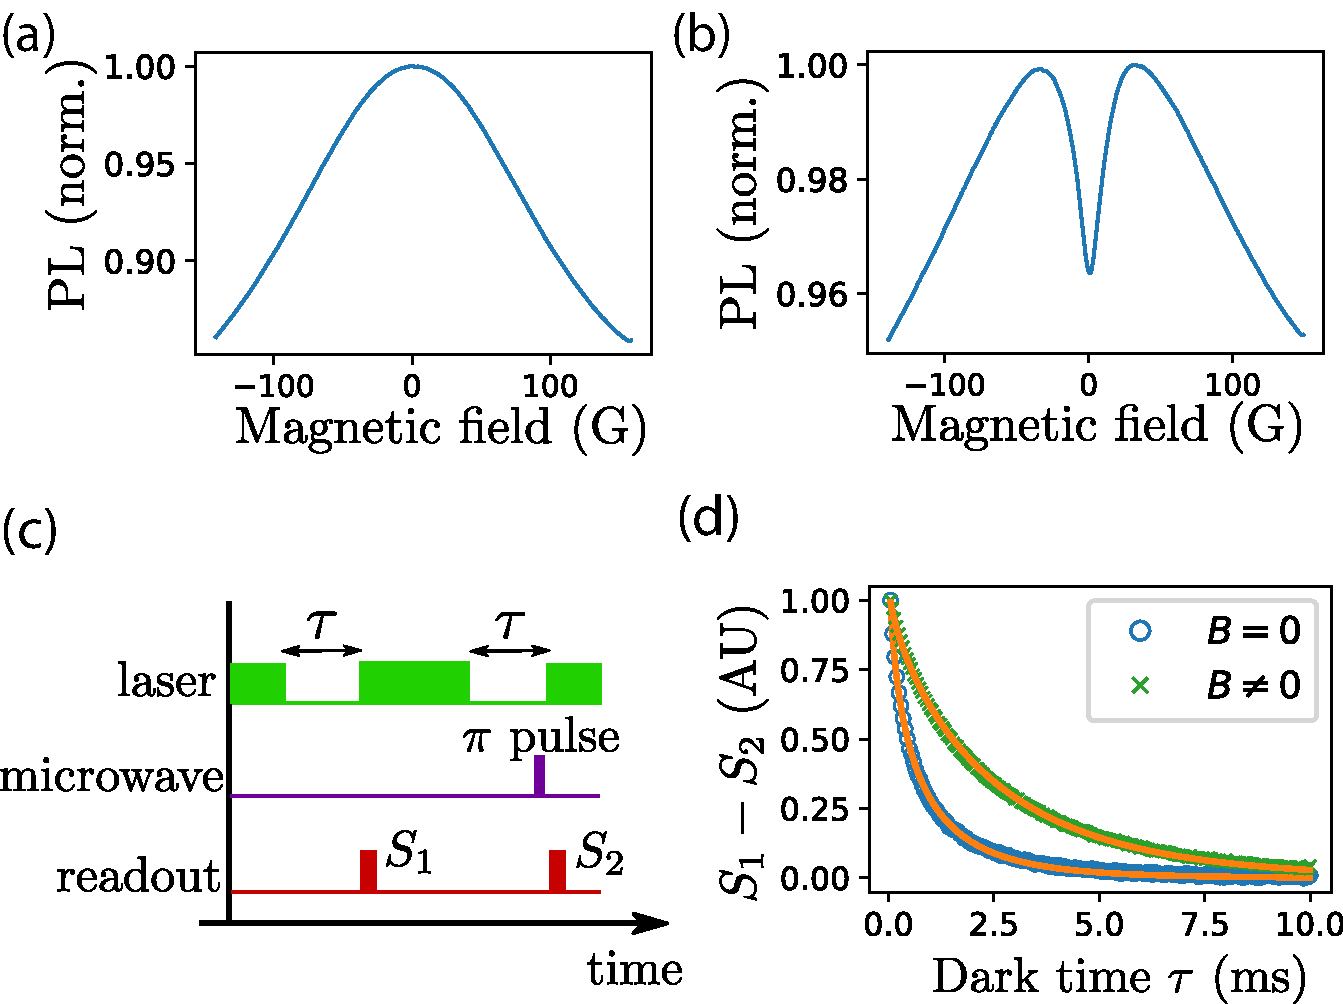
\includegraphics[width=0.45\textwidth]{fig_T1.pdf}
\caption{a) and b) : Photoluminescence from NV center ensembles as a function of a magnetic field applied in an arbitrary direction for sample CVD-1 with [NV$^-$]$\approx 50\ \rm ppb$ and for sample HPHT-150-1 with [NV$^-$]$\approx 3\ \rm ppm$ respectively. (c) Sequence used to measure the spin lifetime. (d) Trace i) and ii) are the spin relaxation signals $S_1-S_2$ measured for the dense sample at zero and non-zero magnetic fields respectively. The fitting procedure (orange plain line) is described in the main text.}
\label{T1}
\end{figure}

\begin{figure*}
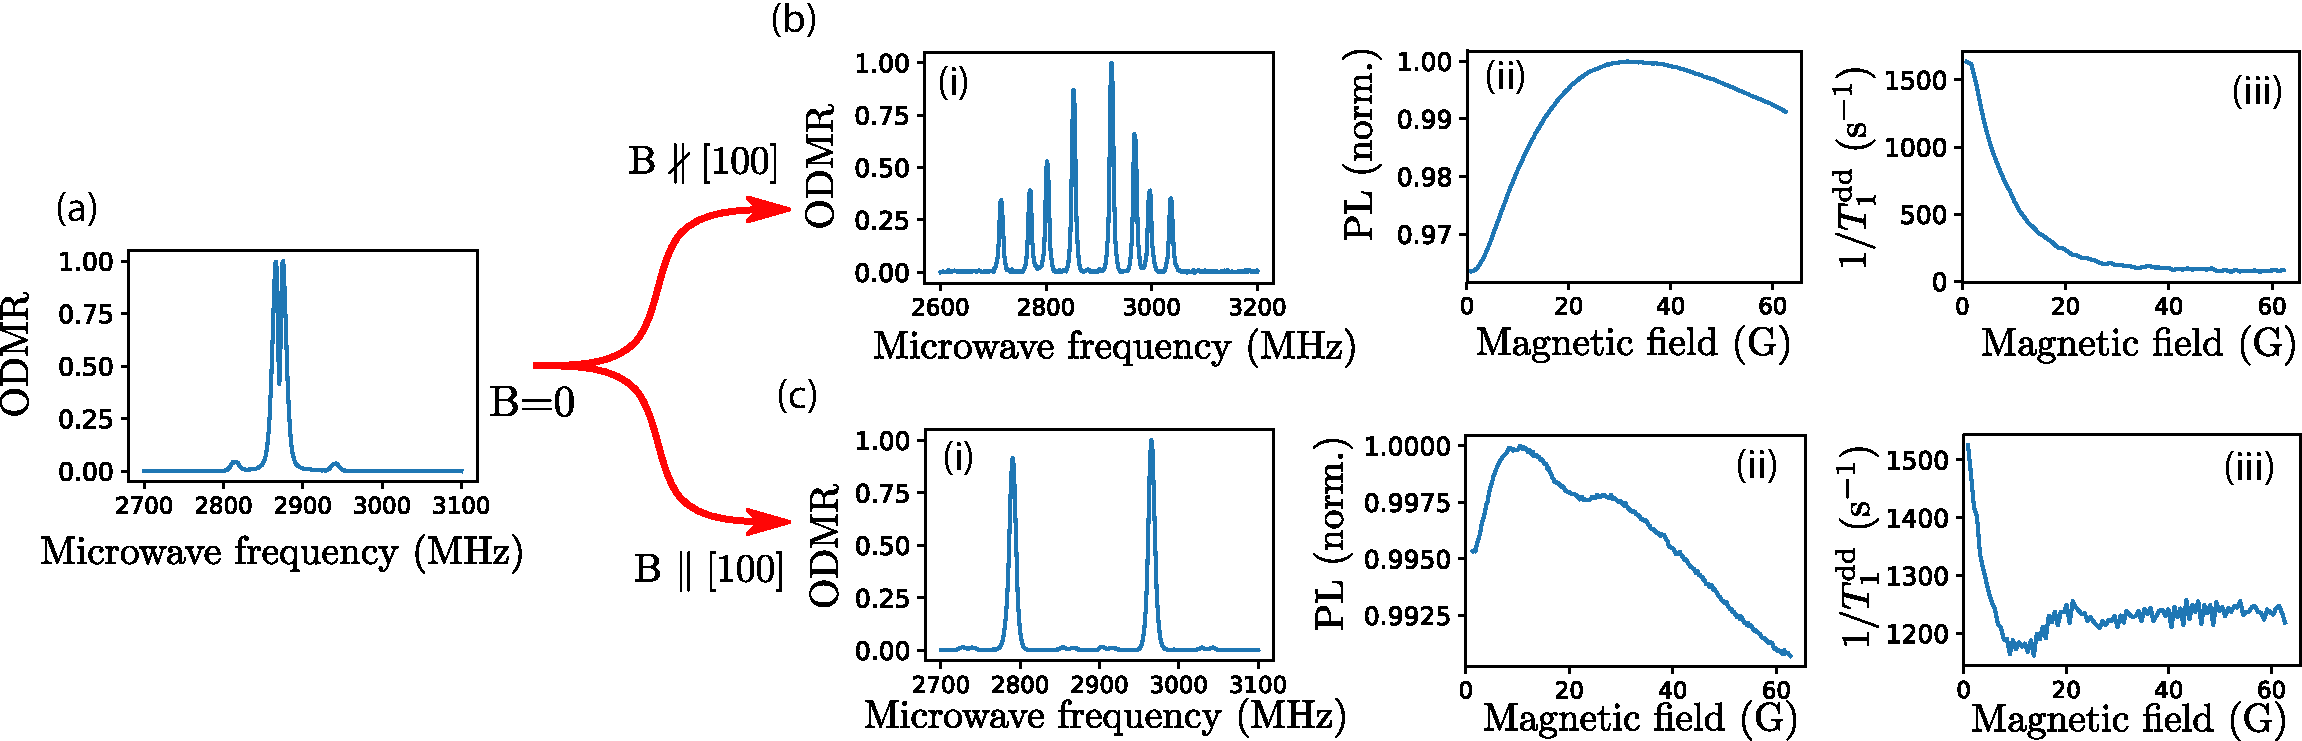
\includegraphics[width=.95\textwidth]{fig_100_vs_1x1x1x1.pdf}
\caption{(a) ODMR spectrum in zero field with microwave amplitude modulation (see experimental details in SM sec. III). (b)-i) ODMR spectrum for a magnetic field $\approx$ 60 G, misaligned by $\sim  24^\circ$ from the [100] axis. (b)-ii) Normalized PL of the NV$^-$ ensemble as a function of the magnetic field amplitude. (b)-iii) Stretched part of the spin decay $1/T_1^{\rm dd}$ as a function of the magnetic field amplitude. (c)-i), (c)-ii) and (c)-iii): same measurements as (b) but with a magnetic field close to the [100] axis. All the measurements were realized using the sample HPHT-150-1.}
\label{100_VS_1x4}
\end{figure*}
%This effect can be observed on all our samples whenever the NV concentration lies in the ppm range. The drop of the PL at low magnetic field was shown to be associated with a decrease of the NV's spin lifetime $T_1$ \citep{jarmola_temperature-_2012}, which results in a decrease of the population in the bright state $\ket{0}$.
%The depolarization dynamics of the NV spins for single or dilute ensembles of NV centers at room temperature is dominated by two-phonon Raman processes \citep{redman1991spin,jarmola_temperature-_2012,norambuena2018spin}, which depend on the crystal lattice temperature. It has been observed that dense NV centers ensembles in fact  have an additional spin decay channel \citep{jarmola_temperature-_2012,jarmola_longitudinal_2015,mrozek_longitudinal_2015, choi2017depolarization, akhmedzhanov_microwave-free_2017, akhmedzhanov_magnetometry_2019, pellet2021magnetic, mrozek2021characterization}, which depends greatly on the magnetic field amplitude. 
This effect has been attributed to CR between the NV centers through dipole-dipole coupling \citep{mrozek_longitudinal_2015, choi2017depolarization}. 
%The reason is that at zero-field all the NV ``classes" - the physical orientation of the NV axes - become resonant, which increases the dipolar relaxation.
%Inhomogeneity of the spin lifetimes is further needed to explain the depolarization of the spin ensemble \citep{choi2017depolarization}. 
We will denote $T_1^{\rm ph}$ the characteristic timescale of phonon-induced relaxation and $T_1^{\rm dd}$ the density dependent timescale associated with dipole-dipole  interactions.
%Before analyzing the cause of low-field depolarization, we present relaxation measurements on HPHT-150-1. Fig. \ref{T1}-c) shows the sequence employed for measuring $T_1^{\rm dd}$. 
Fig. \ref{T1}-c) shows the sequence employed to measure $T_1$ and Fig. \ref{T1}-d) shows the result of the measurement when $B\approx 0$ and $B \approx 50\ \rm G$.
%It consists in a pump-probe measurement where the spins are first polarized in the $\ket{0}$ state by a green laser, and read-out optically after a variable dark time $\tau$. In highly doped samples, this sequence often results in artifacts, mostly due to charge state transfer in the dark \citep{giri_coupled_2018, giri_selective_2019, choi2017depolarization}. It is therefore convenient to repeat the sequence with an additional $\pi$ pulse right on one of the eight NV spin-resonances before the spin read-out to prepare the remaining $\ket{0}$ polarization into a darker $\ket{+1}$ or $\ket{-1}$ state \citep{jarmola_temperature-_2012,mrozek_longitudinal_2015,choi2017depolarization}. By subtracting the result of the two sequences, we select only the spin-dependent part of the signal, with the added benefit of selecting a specific class of NV centers. 
%The relaxation rate is markedly different in both magnetic field settings, with a much more pronounced depolarization at zero-field.
%Notably, the ensemble spin decay curves are not exponential. This was found to be due to inhomogeneities between the spin lifetimes of dipolar coupled NV$^-$ centers \citep{choi2017depolarization}.
%We will interprate our experimental results using the NV-fluctuator model developed in \citep{choi2017depolarization}. This model is based on the existence of very short-lived NV centers - the so-called fluctuators - which, when coupled resonantly to the other NV centers, act as a polarization drain for the spin ensemble. A conclusion of this model is that, for a homogeneous 3D distribution of fluctuators, the dipole-induced relaxation should be a stretched-exponential with a stretch factor $\beta=1/2$. Such a trend was indeed observed when $T_1^{\rm dd} \ll T_1^{\rm ph}$ \cite{choi2017depolarization}. 
%We conducted measurements to confirm the stretch nature of the dipole-induced decay (see SM sec. IV A), as well as confirming the lifetime-limited model of the fluctuators(see SM sec. IV B).
All dense samples used in this study show $T_1^{\rm dd} \sim T_1^{\rm ph}$ (see SM sec. IV A), so both decay processes are included in the analysis. Fitting the two traces of Fig. 2 d) by the product of a simple and a stretched exponential, we find $T_1^{\rm ph}=3.6$ ms for both curves and $T_1^{\rm dd}= 0.6\ \rm ms$ and $13.0\ \rm ms$ for trace i) and ii) respectively. These results thus demonstrates a twenty-fold increase in the dipolar depolarization rate when the B field is turned to zero.
The fluctuator model developed in \citep{choi2017depolarization} contains some of the explanation for this increase in dipolar depolarization: all four NV classes in the diamond are resonant in zero field, which increases the flip-flop rates. However, the model did not include extra specificities in the zero magnetic field region, namely the role of local electric field and double flip processes. 

%We therefore decided to conduct more in depth experiments in order to characterize these potential extra relaxation processes.

Fig. \ref{100_VS_1x4}-a) and b)-i) show optically detected magnetic resonance (ODMR) spectra with and without magnetic field, from the dense ensemble HPHT-150-1. From the resonance line-widths in a magnetic field, we extract decoherence rates $T_2^*$ in the hundreds of nanosecond range, limited by the coupling between NV centers and the fluctuating spins of substitutional nitrogen atoms (also called $P_1$ centers).
%Fig. \ref{100_VS_1x4} (b)-i) shows an ODMR spectrum from the same sample, in a magnetic field. The observed lines correspond to the projections of the magnetic fields onto the four classes of NV centers together with the $\ket{0}\to\ket{-1}$ and $\ket{0}\to\ket{+1}$ spin transitions.
%The transitions frequencies of the four different NV classes are determined by the amplitude and orientation of the external magnetic field.
Using the same magnetic field alignment, Fig. \ref{100_VS_1x4} (b)-ii) and iii) show the PL and the $1/ T_1^{\rm dd}$ decay rates from the NV center ensemble as a function of the amplitude of the magnetic field. 
We observe that the 4~\% increase in PL as the magnetic field increases is indeed correlated with a drop in the spin decay rate from 1600~s$^{-1}$ to 80~s$^{-1}$. This result can again be explained by the decreasing number of resonant spins as the zero magnetic field is increased. We also confirmed that the half width of the dip ($\approx 10$~G) is consistent with a fluctuator model taking into account the reduction of the two spin resonances overlap as the $B$ field is increased (see SM sec. IV C).
%Note that the decrease in PL for $B>40\ \rm G$ is related to state mixing by the transverse magnetic field, so it is not associated with a modification of the spin lifetime. 

Fig. \ref{100_VS_1x4} (c)-i) instead shows an ODMR where all four classes are brought to resonance by placing the magnetic field along the [100] crystalline axis. Fig. \ref{100_VS_1x4} (c)-ii) and (c)-iii) show the change in the PL and in $1/T_1^{\rm dd}$ as a function of a magnetic field that is aligned in this direction. Surprisingly, we can still observe an increase in the spin decay rate and a corresponding drop in the PL when the magnetic field tends to zero, although all classes are always resonant (see SM, sec. IV-E).
We also note that the PL and $1/T_1^{\rm dd}$ change is also much sharper in this scenario.
%One of the main results of this paper is the observation of spin decay in this second scenario and the study on its impact on zero-field magnetometry. 
%Note that the slight drop in PL and the corresponding bump for $1/T_1^{\rm dd}$ at $B \sim 20$G is related to dipolar interaction with NV centers that have a $^{13}$C as a first neighbor \cite{pellet2021optical}. 

When $\gamma | \mathbf{B} |\gg 1/T_2^*$, the only resonant terms in the dipole-dipole coupling between NV centers are the flip-flop terms $~\ket{0,\pm 1}\bra{\pm 1,0}$ (see SM sec. V).
In zero magnetic field however, other resonant mechanisms of the dipolar Hamiltonian have to be taken into consideration, which may elucidate the above result.
It was shown in  \cite{mittiga2018imaging} that local electric fields coming from $P_1^+$ or NV$^-$ centers are responsible for ODMR profiles at zero magnetic field. %Magnetic field noise comes in to second order in zero field. 
In order to estimate their contributions in the spin relaxation, we perform numerical simulations where we add the following Hamiltonian for the electric field dependent NV$^-$ ground state: 
\begin{equation}
\label{NV Hamiltonian}
\mathcal{H}_{\rm elec}= d_\perp \left[ E_x(\hat S_y^2-\hat S_x^2) + E_y(\hat S_x \hat S_y+\hat S_y \hat S_x) \right].
\end{equation}
$E_{x,y}$ are the projections of local electric fields on the NV axes and $d_\perp=17~$Hz $\cdot$ cm/V is the transverse electric field susceptibility. 
Under local electric fields with orientations given by the angle $\phi_E={\rm tan}(E_x/E_y)$, the eigenstates of the total hamiltonian of the NV spins in the ground state are $\ket{0}$ and $\ket{\pm}=\frac{1}{\sqrt{2}}(\ket{+1}\pm e^{-i\phi_E}\ket{-1})$.
Computing the influence of the flip-flop terms $\ket{\pm,0} \bra{0,\pm} $ in the fluctuator model shows that $1/T_1^{\rm dd}$ indeed increases at zero field, even after averaging over all possible angles $\phi_E$ (see SM, sec. V-E).  Another mechanism at stake when considering dipolar interactions between spin-1 systems at low fields are double-flip processes. 
These processes correspond to the terms $\ket{+1,0} \bra{0,-1}$ in the dipolar interaction, giving rise to an exchange of two units of spin-angular momentum when the $\ket{\pm 1}$ states are resonant. Simulations (see SM, sec V-F) suggest that double-flips contribute significantly to the spin relaxation at low fields.
%These processes can become significant when the states $\ket{m_s=\pm 1}$ are degenerate and are thus likely to explain part of the zero-field dip in Fig. 3-c)-ii). 

\begin{figure}
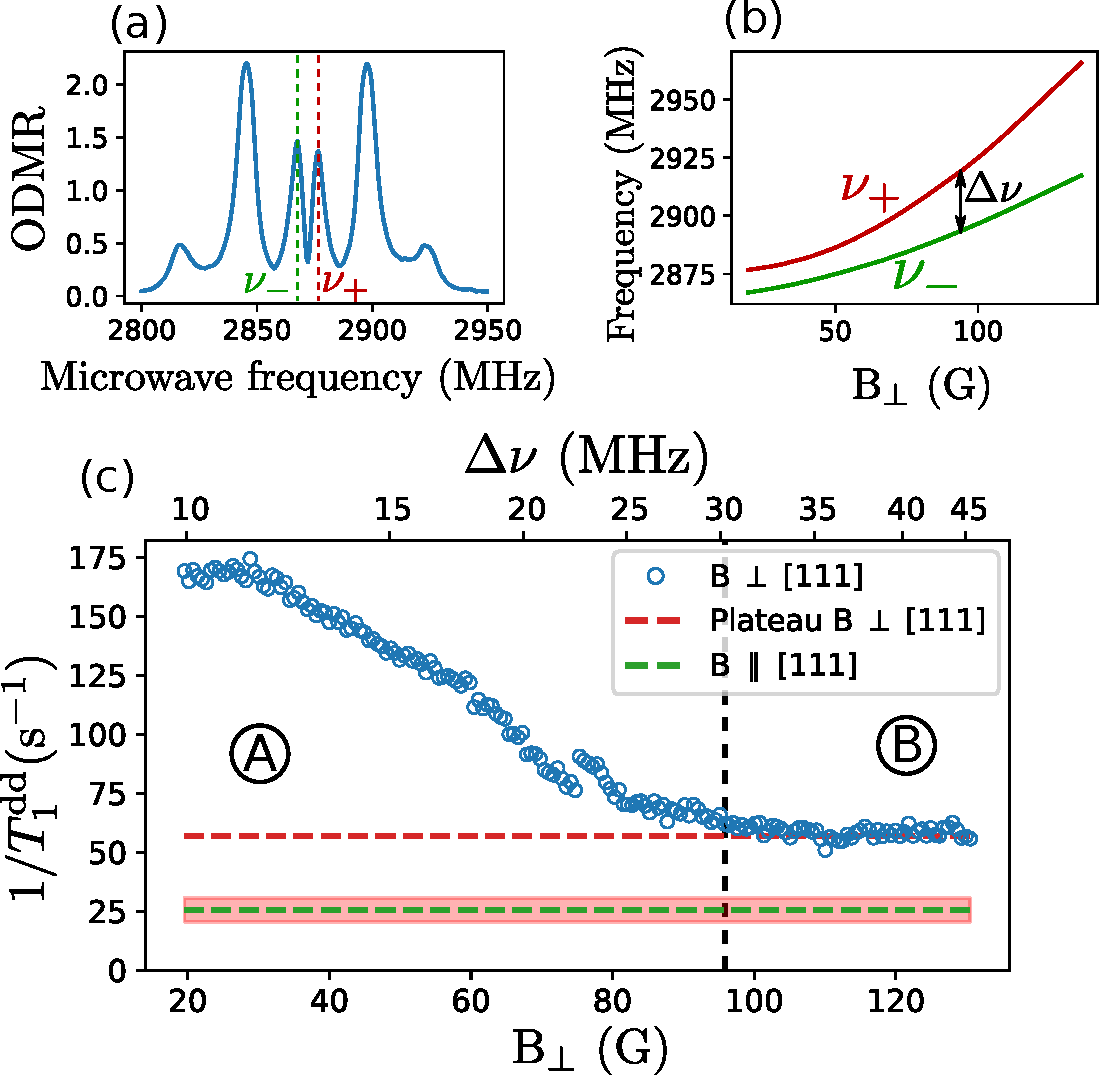
\includegraphics[width=0.45\textwidth]{fig_transverse_field_V3.pdf}
\caption{(a) ODMR spectrum for $B_\perp=20\ \rm G$. The two transition frequencies of the class that is orthogonal to $B$ are denoted $\nu_+$ and $\nu_-$. (b) Measurement of $\nu_+$ and $\nu_-$ through ODMR as a function of $B_\perp$. (c) Measurement of $1/T_1^{\rm dd}$ for a single NV class as a function of $B_\perp$. The red dashed line is the value reached for high transverse field. The green dashed line correspond to the value found for the same sample and NV class, under a longitudinal magnetic field. Error bars are depicted by the shaded pink region. The detuning $\Delta \nu = \nu_+-\nu-$ is indicated on the top $x$-axis. Vertical black dashed line indicates the separation between regions A and B (see main text).}
\label{B_transverse}
\end{figure}

%In order to experimentally discriminate the contribution from the electric field and the double flips, one solution is to apply an electric field in order to lift the degeneracy between the $\ket{+}$ and $\ket{-}$ states. We estimated that, in our samples, we would need a field of $\sim 10^6\ \rm{V/cm}$, which is technically very challenging. 
To quantify these two processes experimentally, we apply a purely transverse magnetic field on one of the NV class. Indeed, when $B_{\perp} \leq 150\ \rm G$, the eigenstates of the spin Hamiltonian are close to $\ket{0}$, $\ket{+}$ and $\ket{-}$ to $\approx 2\%$ (see SM sec. IV-F). We can thus use the transverse field to emulate the role of the electric field, a property that has previously been used to increase the electric field sensing ability of NV centers \cite{dolde2011electric,qiu2022nanoscale}.
Fig.~\ref{B_transverse} (a) shows an ODMR spectrum where $B_{\perp}=20\ \rm G$ on sample HPHT-150-2. The central two lines correspond to the $\ket{0}\to \ket{-}$ and $\ket{0}\to \ket{+}$ transitions for the class that is orthogonal to $\bm B$.
%the other features corresponding to the transitions of the other classes. 
%We chose the initial value of 20 G so that the class of interest is detuned far enough from the other classes. We can therefore safely neglect inter-class flip-flops. 
Fig. \ref{B_transverse}-(c) shows the measurement of the decay rate $1/T_1^{\rm dd}$ for that class, as a function of $B_{\perp}$. Two regions can be observed on this graph: in region A the decay rate decreases with $B_{\perp}$, while in region B it stabilizes to a value $1/T_1^{\rm dd}=60\pm 5\ \rm{s}^{-1}$. We also indicated the value $1/T_1^{\rm dd}=25\pm 5\ \rm{s}^{-1}$ found for the same class but employing a longitudinal magnetic field. % instead of transverse to it.


\begin{figure}[ht]
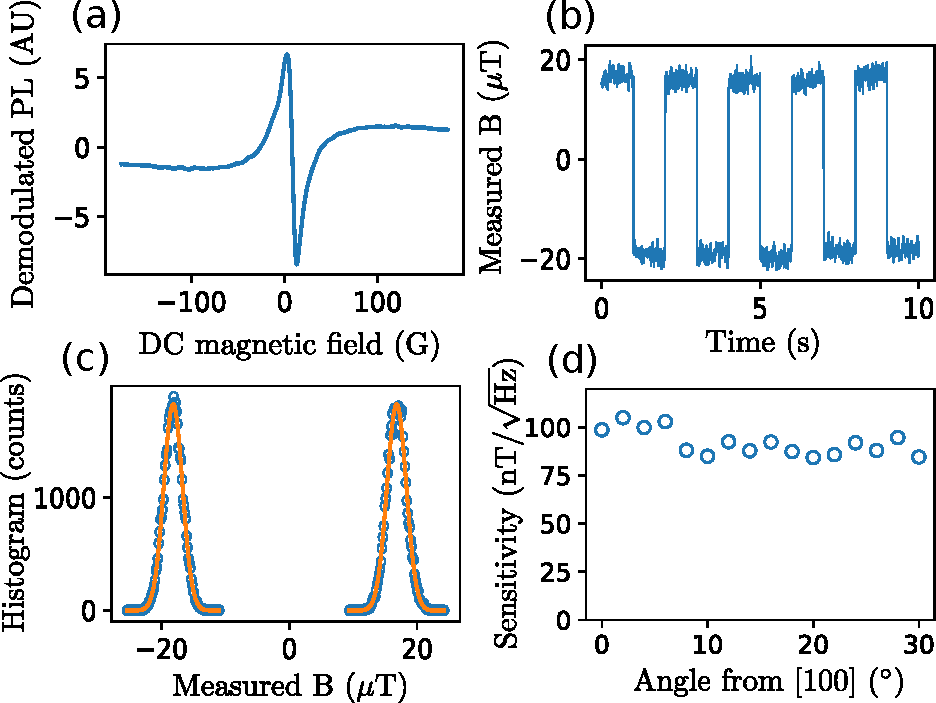
\includegraphics[width=0.45\textwidth]{fig_magneto}
\caption{Low-field magnetometry protocol. (a) Demodulated PL as a function of an externally applied magnetic field. (b) External magnetic field read-out. (c) Histogram of the measurement in Fig. (b) fitted by gaussians of standard deviation $\sigma=1.5\ \mu \rm T$. (d) Measured sensitivity as function of the angle between the external magnetic field and the [100] crystalline axis.}
\label{magneto}
\end{figure}


To understand these results, we plot the detuning $\Delta \nu$ between the states $\ket{+}$ and $\ket{-}$ as a function of $B_{\perp}$ in Fig. \ref{B_transverse} (b). When $\delta \nu > 1/T_2^*$, these states do not overlap any longer, so we can interpret our results as follows: double-flips are efficient in region A, up to a point where state overlap is negligible. In region B, only the flip-flops in the basis $\ket{\pm}$ play a role. We note that the decay rate in the $\{ \ket{0}, \ket{\pm} \}$ basis is more than a factor of two larger than the decay rate coming from intra-class flip-flops in the $\{\ket{0}, \ket{\pm 1} \}$ basis. This effect is corroborated by our model detailed in SM sec. V. Importantly, in region A, the double-flips processes give a maximum decay rate that is $\sim 5$ times greater than the decay caused by the change of basis alone. From these results and according to our model, the double-flips are thus the dominant cause of zero-field depolarization observed in Fig. \ref{100_VS_1x4} (c)-iii).

Our observations have important implications for magnetometry with NV ensembles.
DC microwave-free magnetometry has already been performed using either NV-NV cross-relaxations \citep{akhmedzhanov_microwave-free_2017,akhmedzhanov_magnetometry_2019} or level anti-crossing \citep{Wickenbrock, zheng2017level, zheng_microwave-free_2020}. Here we propose a similar protocol but using the spin depolarization at zero-field. 
To do so, we use a lock-in detection and add a magnetic field modulation at $\sim 1\ \rm kHz$ with an amplitude $\sim 10\ \rm G$ through the same electromagnet. Fig. \ref{magneto}-(a) shows the demodulated PL while a DC magnetic field is scanned in an arbitrary direction. Here, we use the sample HPHT-15-1 with a laser power $\sim 1\ \rm mW$. The optical power in the collected PL is $\sim 1\ \mu\rm W$.  We can see a sharp linear slope in low field $\abs{B} < 5\ \rm G$. Once calibrated, the slope provides a 1D magnetometer, which could be extended to 3D with a set of 3 coils or 3 electromagnets, as in \cite{zheng_microwave-free_2020}. In order to assess the sensitivity of the measurement, we alternate a small DC field of $\approx 40\ \mu\rm{T}$ every few seconds and take a histogram of the measured fields (with a total duration of $\approx $50 s), as shown in Fig. \ref{magneto}-(b) and (c). The histogram is well fitted by gaussians of standard deviation $\sigma=1.5\ \mu \rm T$. The measurement was performed here with an output low-pass filter of time constant $\tau=3\ \rm ms$, which gives us a DC sensitivity $\eta=\sigma \sqrt{\tau}=82\ \rm{nT}/\sqrt{\rm Hz}$. This value corresponds to $\eta/\sqrt{V}\approx 4.7 \ \mu \rm{T}/\mu m^{3/2}/\sqrt{\rm Hz}$ when normalized to the volume. Importantly, this measurement is consistent with the experimentally found $\sim 5\ \mu \rm{T}/\sqrt{\rm Hz}$ sensitivity obtained with sample HPHT-1-1 (see samples details in SM sec. II). 

Our results implies bright perspectives for high-sensitivity magnetometry using NV centers in a millimeter size volumes. Furthermore, compared to previously employed protocols, the sensitivity does not crucially depend on crystalline orientation, making this magnetometer principle operational with diamond powders or polycrystalline samples. Another significant advantage is that this measurement is insensitive to thermal fluctuations and strain inhomogeneities because dipolar-relaxation at zero-field does not depend on the zero-field splitting. In other typical NV magnetometers however, the zero-field splitting dependence with temperature and strain can give systematic errors \cite{Bauch, Barry}. 


We now evaluate the relative role of the three causes of spin depolarization that assist the operation of the magnetometer. To do so, we measure its sensitivity while changing the angle of the magnetic field.  The results are shown in Fig. \ref{magneto} (d). We observe only a $\sim$ 10\% improvement in the sensitivity as we leave the [100] region.
When $\bm B \parallel [100]$ only the double flips and the electric field cause a depolarization, whereas the three effects are at play in all the other orientations. It should be noted that this observation is sample dependent. Other samples, including those from the same batch, have shown a higher orientation dependence, corresponding to a lower contribution from local electric fields and double-flip processes.
Interestingly, the double-flips and electric field effects are here the dominant factors in the sensitivity of this protocol. 
%It may seem surprising at first that the effects with a lower contribution to the PL contrast have a higher effect on this PL-based protocol. The reason why this is the case is that the slope of the change of contrast with respect to the magnetic field is larger when depolarization is caused by local electric fields and double-flips processes than solely by flip-flops processes.   

As a conclusion, we identified three mechanisms causing spin depolarization in zero field for dense ensemble of NV$^-$ centers, all related to an increase in the dipole-dipole induced CR between the spins of NV centers. The lift in degeneracy of the spin state of different NV classes was found to be the main cause of zero-field depolarization, followed by double-flip processes and then the electric field induced mixing. We have employed CR for microwave and orientation-free DC-magnetometry and demonstrated a sensitivity below $100\ \rm{nT}/\sqrt{\rm Hz}$ for a single $15\ \mu \rm m$ diameter commercially available diamond and show that that double-flips and local electric fields play a critical role. 
We believe that our results will also be important for microwave-based low field magnetometry \cite{Vetter_LFM, WangRB} and for understanding many-body phenomena \citep{kucsko2018critical, ChoiNat, ZuYao, dwyer2021probing} and spin-mechanical effects \cite{pellet2021magnetic} with strongly coupled spins under purely transverse or small magnetic fields. 

\begin{acknowledgments}

We would like to acknowledge support from Alexandre Tallaire and Jocelyn Achard as well as 
SIRTEQ for funding.

\end{acknowledgments}
\bibliographystyle{apsrev4-2}
\bibliography{CR}{}




\end{document}